\documentclass[11pt, a4paper]{article}

% Fonts and Encoding
\usepackage[utf8]{inputenc}
\usepackage[T1]{fontenc}
\usepackage{lmodern}

% Math and Symbols
\usepackage{amsmath, amssymb, amsthm, amsfonts, mathrsfs, mathtools}

% Layout and Geometry
\usepackage{geometry}
\geometry{a4paper, margin=1in}

% Formatting and Graphics
\usepackage{graphicx, xcolor, enumitem, booktabs, array, tabularx}

% TikZ for Illustrations
\usepackage{tikz}
\usetikzlibrary{arrows.meta, positioning, shapes.geometric, calc, backgrounds, matrix}

% Clickable Links and TOC
\usepackage{hyperref}
\hypersetup{
    colorlinks=true,
    linkcolor=blue,
    filecolor=magenta,      
    urlcolor=cyan,
    pdftitle={Congruence Modulo n and Equivalence Relations},
}

% Theorem Environments
\newtheorem{theorem}{Theorem}[section]
\newtheorem{lemma}[theorem]{Lemma}
\newtheorem{proposition}[theorem]{Proposition}
\newtheorem{corollary}[theorem]{Corollary}
\theoremstyle{definition}
\newtheorem{definition}{Definition}[section]
\newtheorem{axiom}{Axiom}[section]
\newtheorem{example}{Example}[section]
\theoremstyle{remark}
\newtheorem{remark}{Remark}[section]

% Custom Commands (Enforced standard notation)
\newcommand{\R}{\mathbb{R}}
\newcommand{\N}{\mathbb{N}}
\newcommand{\Z}{\mathbb{Z}}
\newcommand{\Q}{\mathbb{Q}}
\newcommand{\E}{\mathbb{E}}
\newcommand{\Prob}{\mathbb{P}}
\newcommand{\F}{\mathcal{F}}

\begin{document}

\title{\textbf{Advanced Abstract Mathematics: \\ Congruence Modulo $n$ and Equivalence Relations}}
\author{Tashfeen Omran}
\date{}
\maketitle

\tableofcontents
\newpage

% ==========================================
% PART 1: INTRODUCTION
% ==========================================
\section{Part 1: Comprehensive Introduction, Context, and Prerequisites}

\subsection{Core Concepts \& Axioms}
In the study of abstract algebra and number theory, one of the most foundational structures is the concept of \textbf{Congruence Modulo $n$}. It serves as the prototypical example of an equivalence relation, bridging the gap between basic arithmetic and advanced quotient spaces. 

\begin{definition}[Congruence Modulo $n$]
Let $n \in \mathbb{Z}$ such that $n \geq 2$. For any two integers $a, b \in \mathbb{Z}$, we say that $a$ is congruent to $b$ modulo $n$, denoted as:
\[ \displaystyle a \equiv b \pmod{n} \]
if and only if $n$ divides the difference $(a - b)$. Formally, this means there exists some integer $k \in \mathbb{Z}$ such that $a - b = kn$.
\end{definition}

This definition establishes a relation on the set of integers $\mathbb{Z}$. An \textbf{Equivalence Relation} (typically denoted by $\sim$ or $R$) on a set $A$ is a relation that satisfies three axiomatic properties:
\begin{enumerate}
    \item \textbf{Reflexivity:} For all $a \in A$, $a \mathrel{R} a$.
    \item \textbf{Symmetry:} For all $a, b \in A$, if $a \mathrel{R} b$, then $b \mathrel{R} a$.
    \item \textbf{Transitivity:} For all $a, b, c \in A$, if $a \mathrel{R} b$ and $b \mathrel{R} c$, then $a \mathrel{R} c$.
\end{enumerate}

When a relation satisfies these three properties, it partitions the underlying set into disjoint subsets called \textbf{Equivalence Classes}. The equivalence class of an element $a$, denoted $[a]$, is the set of all elements related to $a$:
\[ \displaystyle [a] = \{ x \in A \mid x \mathrel{R} a \} \]

\subsection{Intuition and Set-Theoretic Foundations}
Intuitively, congruence modulo $n$ is "clock arithmetic." On a standard 12-hour clock, 13:00 is equivalent to 1:00 because $13 - 1 = 12$, which is a multiple of 12. Set-theoretically, the relation $a \equiv b \pmod{n}$ groups all integers that leave the same remainder when divided by $n$ into the same subset. These subsets are mutually exclusive and collectively exhaustive, meaning they form a perfect \textbf{partition} of $\mathbb{Z}$. The set of all such equivalence classes is denoted as $\mathbb{Z}_n$ (or $\mathbb{Z}/n\mathbb{Z}$), representing a fundamental quotient space.

\subsection{Historical Context and Motivation}
The formalization of modular arithmetic was introduced by Carl Friedrich Gauss in his seminal 1801 work, \textit{Disquisitiones Arithmeticae}. Before Gauss, mathematicians studied divisibility on an ad-hoc basis. Gauss realized that by treating "congruence" as a form of equality, one could perform algebraic manipulations (addition, multiplication) on the remainders themselves. This paradigm shift laid the groundwork for modern abstract algebra, cryptography (such as RSA), and computer science.

\subsection{Key Theorems}
\begin{theorem}[Congruence is an Equivalence Relation]
Let $n \in \mathbb{Z}$ with $n \geq 2$. The relation $R$ defined on $\mathbb{Z}$ by $a \mathrel{R} b$ if $a \equiv b \pmod{n}$ is an equivalence relation.
\end{theorem}

\subsection{Prerequisites}
To master this section, the reader must be fluent in:
\begin{itemize}
    \item \textbf{Divisibility Rules:} Understanding that $a \mid b$ implies $b = ak$ for some integer $k$.
    \item \textbf{Direct Proof Techniques:} Constructing logical chains from definitions to conclusions.
    \item \textbf{Set Theory Basics:} Understanding unions, intersections, and partitions of sets.
\end{itemize}

\newpage
% ==========================================
% PART 2: DETAILED HOMEWORK SOLUTIONS
% ==========================================
\section{Part 2: Detailed Homework Solutions (Rigorous Proofs \& Computations)}

\subsection*{Exercise 9.44}
\textbf{Problem:} Classify each of the following statements as true or false.
(a) $25 \equiv 9 \pmod{8}$, (b) $-17 \equiv 9 \pmod{8}$, (c) $-14 \equiv -14 \pmod{4}$, (d) $25 \equiv -3 \pmod{11}$.

\textbf{Solution:}
We use the definition: $a \equiv b \pmod{n} \iff n \mid (a - b)$.
\begin{itemize}
    \item \textbf{(a)} $25 - 9 = 16$. Since $16 = 8(2)$, $8 \mid 16$. \textbf{True.}
    \item \textbf{(b)} $-17 - 9 = -26$. Since $-26 / 8 = -3.25 \notin \mathbb{Z}$, $8 \nmid -26$. \textbf{False.}
    \item \textbf{(c)} $-14 - (-14) = 0$. Since $0 = 4(0)$, $4 \mid 0$. \textbf{True.}
    \item \textbf{(d)} $25 - (-3) = 28$. Since $28 / 11 \notin \mathbb{Z}$, $11 \nmid 28$. \textbf{False.}
\end{itemize}

\subsection*{Exercise 9.45}
\textbf{Problem:} A relation $R$ is defined on $\mathbb{Z}$ by $a \mathrel{R} b$ if $3a + 5b \equiv 0 \pmod{8}$. Prove that $R$ is an equivalence relation.

\textbf{Proof (Direct Proof):}
We must show that $R$ is reflexive, symmetric, and transitive.
\begin{enumerate}
    \item \textbf{Reflexive:} Let $a \in \mathbb{Z}$. We evaluate $3a + 5a = 8a$. Since $8a = 8(a)$ and $a \in \mathbb{Z}$, it follows that $8 \mid (3a + 5a)$. Thus, $3a + 5a \equiv 0 \pmod{8}$, meaning $a \mathrel{R} a$. $R$ is reflexive.
    \item \textbf{Symmetric:} Let $a, b \in \mathbb{Z}$ and assume $a \mathrel{R} b$. By definition, $3a + 5b \equiv 0 \pmod{8}$, which means $3a + 5b = 8k$ for some $k \in \mathbb{Z}$. We must show $b \mathrel{R} a$, meaning $3b + 5a \equiv 0 \pmod{8}$. 
    Observe the sum of the two expressions:
    \[ \displaystyle (3a + 5b) + (5a + 3b) = 8a + 8b = 8(a + b) \]
    Isolating the target expression yields:
    \[ \displaystyle 5a + 3b = 8(a + b) - (3a + 5b) = 8(a + b) - 8k = 8(a + b - k) \]
    Since $(a + b - k) \in \mathbb{Z}$, $8 \mid (5a + 3b)$. Thus, $b \mathrel{R} a$. $R$ is symmetric.
    \item \textbf{Transitive:} Let $a, b, c \in \mathbb{Z}$. Assume $a \mathrel{R} b$ and $b \mathrel{R} c$. Then there exist $k, j \in \mathbb{Z}$ such that:
    \[ \displaystyle 3a + 5b = 8k \quad \text{and} \quad 3b + 5c = 8j \]
    Adding these two equations gives:
    \[ \displaystyle (3a + 5b) + (3b + 5c) = 8k + 8j \implies 3a + 8b + 5c = 8(k + j) \]
    Subtracting $8b$ from both sides yields:
    \[ \displaystyle 3a + 5c = 8(k + j - b) \]
    Since $(k + j - b) \in \mathbb{Z}$, $8 \mid (3a + 5c)$. Thus, $a \mathrel{R} c$. $R$ is transitive.
\end{enumerate}
Since $R$ is reflexive, symmetric, and transitive, it is an equivalence relation. $\blacksquare$

\subsection*{Exercise 9.46}
\textbf{Problem:} Let $R$ be the relation defined on $\mathbb{Z}$ by $a \mathrel{R} b$ if $a + b \equiv 0 \pmod{3}$. Show that $R$ is not an equivalence relation.

\textbf{Proof (Counterexample):}
To show a relation is not an equivalence relation, it suffices to show it fails at least one of the three properties. Let us test reflexivity. For $R$ to be reflexive, $a \mathrel{R} a$ must hold for all $a \in \mathbb{Z}$, meaning $a + a \equiv 0 \pmod{3}$. 
Let $a = 1$. Then $1 + 1 = 2$. Since $3 \nmid 2$, $1 \not\mathrel{R} 1$. 
Because $R$ is not reflexive, it is not an equivalence relation. $\blacksquare$

\subsection*{Exercise 9.47}
\textbf{Problem:} The relation $R$ on $\mathbb{Z}$ defined by $a \mathrel{R} b$ if $a^2 \equiv b^2 \pmod{4}$ is known to be an equivalence relation. Determine the distinct equivalence classes.

\textbf{Solution:}
We must find the possible values of $x^2 \pmod{4}$ for $x \in \mathbb{Z}$. By the Division Algorithm, any integer $x$ can be written as $x = 2k$ (even) or $x = 2k + 1$ (odd).
\begin{itemize}
    \item If $x$ is even, $x = 2k \implies x^2 = 4k^2 \equiv 0 \pmod{4}$.
    \item If $x$ is odd, $x = 2k + 1 \implies x^2 = 4k^2 + 4k + 1 = 4(k^2 + k) + 1 \equiv 1 \pmod{4}$.
\end{itemize}
Thus, $a^2 \equiv b^2 \pmod{4}$ if and only if $a$ and $b$ have the same parity (both even or both odd). 
The distinct equivalence classes are:
\[ \displaystyle [0] = \{ x \in \mathbb{Z} \mid x \text{ is even} \} \]
\[ \displaystyle [1] = \{ x \in \mathbb{Z} \mid x \text{ is odd} \} \]

\subsection*{Exercise 9.48}
\textbf{Problem:} The relation $R$ defined on $\mathbb{Z}$ by $x \mathrel{R} y$ if $x^3 \equiv y^3 \pmod{4}$ is known to be an equivalence relation. Determine the distinct equivalence classes.

\textbf{Solution:}
We evaluate $x^3 \pmod{4}$ for the standard representatives of $\mathbb{Z}_4$:
\begin{align*}
    0^3 &= 0 \equiv 0 \pmod{4} \\
    1^3 &= 1 \equiv 1 \pmod{4} \\
    2^3 &= 8 \equiv 0 \pmod{4} \\
    3^3 &= 27 \equiv 3 \pmod{4}
\end{align*}
Integers $x$ and $y$ are related if their cubes yield the same remainder modulo 4. Based on the above:
\begin{itemize}
    \item Elements congruent to 0 or 2 modulo 4 yield a cube congruent to 0 modulo 4.
    \item Elements congruent to 1 modulo 4 yield a cube congruent to 1 modulo 4.
    \item Elements congruent to 3 modulo 4 yield a cube congruent to 3 modulo 4.
\end{itemize}
Thus, there are three distinct equivalence classes:
\[ \displaystyle [0] = \{ x \in \mathbb{Z} \mid x \equiv 0 \pmod{4} \text{ or } x \equiv 2 \pmod{4} \} = \{ x \in \mathbb{Z} \mid x \text{ is even} \} \]
\[ \displaystyle [1] = \{ x \in \mathbb{Z} \mid x \equiv 1 \pmod{4} \} \]
\[ \displaystyle [3] = \{ x \in \mathbb{Z} \mid x \equiv 3 \pmod{4} \} \]

\subsection*{Exercise 9.49}
\textbf{Problem:} A relation $R$ is defined on $\mathbb{Z}$ by $a \mathrel{R} b$ if $5a \equiv 2b \pmod{3}$. Prove that $R$ is an equivalence relation and determine the distinct equivalence classes.

\textbf{Proof:}
First, observe that $5 \equiv 2 \pmod{3}$. Therefore, the condition $5a \equiv 2b \pmod{3}$ is algebraically equivalent to $2a \equiv 2b \pmod{3}$. Since $\gcd(2, 3) = 1$, we can multiply both sides by the modular inverse of 2 modulo 3 (which is 2, since $2 \times 2 = 4 \equiv 1 \pmod{3}$). 
\[ \displaystyle 2(2a) \equiv 2(2b) \pmod{3} \implies 4a \equiv 4b \pmod{3} \implies a \equiv b \pmod{3} \]
Thus, $a \mathrel{R} b \iff a \equiv b \pmod{3}$. 
Since we already know from Theorem 9.14 that congruence modulo $n$ is an equivalence relation, $R$ is an equivalence relation. 
The distinct equivalence classes are simply the congruence classes modulo 3:
\[ \displaystyle [0] = \{ 3k \mid k \in \mathbb{Z} \}, \quad [1] = \{ 3k + 1 \mid k \in \mathbb{Z} \}, \quad [2] = \{ 3k + 2 \mid k \in \mathbb{Z} \} \]
$\blacksquare$

\subsection*{Exercise 9.50}
\textbf{Problem:} A relation $R$ is defined on $\mathbb{Z}$ by $a \mathrel{R} b$ if $2a + 2b \equiv 0 \pmod{4}$. Prove that $R$ is an equivalence relation and determine the distinct equivalence classes.

\textbf{Proof:}
The condition $2a + 2b \equiv 0 \pmod{4}$ means $4 \mid (2a + 2b)$, which implies $2a + 2b = 4k$ for some $k \in \mathbb{Z}$. Dividing the entire equation by 2 yields $a + b = 2k$. This means $a + b \equiv 0 \pmod{2}$, which is equivalent to saying $a$ and $b$ have the same parity (either both even or both odd). 
Let us verify the properties:
\begin{enumerate}
    \item \textbf{Reflexive:} $a + a = 2a \equiv 0 \pmod{2}$. Thus $a \mathrel{R} a$.
    \item \textbf{Symmetric:} If $a + b \equiv 0 \pmod{2}$, then $b + a \equiv 0 \pmod{2}$. Thus $a \mathrel{R} b \implies b \mathrel{R} a$.
    \item \textbf{Transitive:} If $a + b = 2k$ and $b + c = 2j$, adding them gives $a + 2b + c = 2(k + j) \implies a + c = 2(k + j - b)$. Thus $a + c \equiv 0 \pmod{2}$, so $a \mathrel{R} c$.
\end{enumerate}
$R$ is an equivalence relation. The distinct equivalence classes are based on parity:
\[ \displaystyle [0] = \{ x \in \mathbb{Z} \mid x \text{ is even} \}, \quad [1] = \{ x \in \mathbb{Z} \mid x \text{ is odd} \} \]
$\blacksquare$

\subsection*{Exercise 9.51}
\textbf{Problem:} Let $R$ be the relation defined on $\mathbb{Z}$ by $a \mathrel{R} b$ if $2a + 3b \equiv 0 \pmod{5}$. Prove that $R$ is an equivalence relation and determine the distinct equivalence classes.

\textbf{Proof:}
Notice that $3 \equiv -2 \pmod{5}$. We can rewrite the relation condition as:
\[ \displaystyle 2a - 2b \equiv 0 \pmod{5} \implies 2(a - b) \equiv 0 \pmod{5} \]
Since $\gcd(2, 5) = 1$, we can multiply by the inverse of 2 modulo 5 (which is 3) to cancel the 2:
\[ \displaystyle 3 \cdot 2(a - b) \equiv 3 \cdot 0 \pmod{5} \implies 6(a - b) \equiv 0 \pmod{5} \implies a - b \equiv 0 \pmod{5} \]
Thus, $a \mathrel{R} b \iff a \equiv b \pmod{5}$. By Theorem 9.14, this is the standard congruence modulo 5, which is an equivalence relation. 
The distinct equivalence classes are:
\[ \displaystyle [0], [1], [2], [3], [4] \pmod{5} \]
$\blacksquare$

\subsection*{Exercise 9.52}
\textbf{Problem:} Let $R$ be the relation defined on $\mathbb{Z}$ by $a \mathrel{R} b$ if $a^2 \equiv b^2 \pmod{5}$. Prove that $R$ is an equivalence relation and determine the distinct equivalence classes.

\textbf{Proof:}
\begin{enumerate}
    \item \textbf{Reflexive:} For any $a \in \mathbb{Z}$, $a^2 \equiv a^2 \pmod{5}$. Thus $a \mathrel{R} a$.
    \item \textbf{Symmetric:} If $a^2 \equiv b^2 \pmod{5}$, then $b^2 \equiv a^2 \pmod{5}$. Thus $a \mathrel{R} b \implies b \mathrel{R} a$.
    \item \textbf{Transitive:} If $a^2 \equiv b^2 \pmod{5}$ and $b^2 \equiv c^2 \pmod{5}$, then by the transitivity of standard congruence, $a^2 \equiv c^2 \pmod{5}$. Thus $a \mathrel{R} c$.
\end{enumerate}
$R$ is an equivalence relation. To find the classes, we compute squares modulo 5:
\begin{align*}
    0^2 &\equiv 0 \pmod{5} \\
    1^2 &\equiv 1 \pmod{5} \\
    2^2 &\equiv 4 \pmod{5} \\
    3^2 &\equiv 9 \equiv 4 \pmod{5} \\
    4^2 &\equiv 16 \equiv 1 \pmod{5}
\end{align*}
Elements are related if their squares are congruent. Grouping by the square values $\{0, 1, 4\}$:
\[ \displaystyle [0] = \{ x \in \mathbb{Z} \mid x \equiv 0 \pmod{5} \} \]
\[ \displaystyle [1] = \{ x \in \mathbb{Z} \mid x \equiv 1 \pmod{5} \text{ or } x \equiv 4 \pmod{5} \} \]
\[ \displaystyle [2] = \{ x \in \mathbb{Z} \mid x \equiv 2 \pmod{5} \text{ or } x \equiv 3 \pmod{5} \} \]
$\blacksquare$

\subsection*{Exercise 9.53}
\textbf{Problem:} Define a relation $R$ on the set $\mathbb{R}$ of real numbers by $a \mathrel{R} b$ if $a - b = k\pi$ for some $k \in \mathbb{Z}$. Is this relation $R$ an equivalence relation? If not, explain why. If yes, prove this and determine $[0], [\pi]$ and $[\sqrt{2}]$.

\textbf{Proof:}
We test the three properties of an equivalence relation on $\mathbb{R}$:
\begin{enumerate}
    \item \textbf{Reflexive:} Let $a \in \mathbb{R}$. $a - a = 0 = 0 \cdot \pi$. Since $0 \in \mathbb{Z}$, $a \mathrel{R} a$.
    \item \textbf{Symmetric:} Let $a, b \in \mathbb{R}$ and assume $a \mathrel{R} b$. Then $a - b = k\pi$ for some $k \in \mathbb{Z}$. Multiplying by $-1$ gives $b - a = (-k)\pi$. Since $-k \in \mathbb{Z}$, $b \mathrel{R} a$.
    \item \textbf{Transitive:} Let $a, b, c \in \mathbb{R}$. Assume $a \mathrel{R} b$ and $b \mathrel{R} c$. Then $a - b = k\pi$ and $b - c = j\pi$ for some $k, j \in \mathbb{Z}$. Adding the equations yields $(a - b) + (b - c) = k\pi + j\pi \implies a - c = (k + j)\pi$. Since $(k + j) \in \mathbb{Z}$, $a \mathrel{R} c$.
\end{enumerate}
Yes, $R$ is an equivalence relation. 
The equivalence classes are:
\[ \displaystyle [0] = \{ x \in \mathbb{R} \mid x - 0 = k\pi \} = \{ k\pi \mid k \in \mathbb{Z} \} \]
\[ \displaystyle [\pi] = \{ x \in \mathbb{R} \mid x - \pi = k\pi \} = \{ (k+1)\pi \mid k \in \mathbb{Z} \} = \{ m\pi \mid m \in \mathbb{Z} \} = [0] \]
\[ \displaystyle [\sqrt{2}] = \{ x \in \mathbb{R} \mid x - \sqrt{2} = k\pi \} = \{ \sqrt{2} + k\pi \mid k \in \mathbb{Z} \} \]
$\blacksquare$

\newpage
% ==========================================
% PART 3: IN-DEPTH ANALYSIS
% ==========================================
\section{Part 3: In-Depth Analysis of Problems and Techniques}

\subsection{A) Problem Types and Logical Strategies}
The exercises in Section 9.5 fall into three distinct analytical categories:
\begin{enumerate}
    \item \textbf{Direct Verification of Equivalence Relations (e.g., 9.45, 9.50):} The strategy here is highly mechanical. You must strictly write down the definitions of Reflexivity, Symmetry, and Transitivity, and use algebraic manipulation (usually adding equations or factoring) to show the properties hold.
    \item \textbf{Counterexample Generation (e.g., 9.46):} When a relation is suspected to be false, the most efficient strategy is to test Reflexivity first. Often, relations involving a sum (like $a + b \equiv 0$) fail reflexivity because $a + a = 2a$, which is not universally divisible by the modulus.
    \item \textbf{Equivalence Class Determination (e.g., 9.47, 9.48, 9.52):} The strategy is exhaustive evaluation over the finite quotient space $\mathbb{Z}_n$. Because there are only $n$ possible remainders, you can simply test $0, 1, \dots, n-1$ to see which elements group together under the given mapping (like squaring or cubing).
\end{enumerate}

\subsection{B) Key Analytical and Logical Manipulations}
\begin{itemize}
    \item \textbf{The "Add and Subtract" Trick (Exercise 9.45):} To prove symmetry for $3a + 5b \equiv 0 \pmod{8}$, we needed to evaluate $5a + 3b$. The trick was to recognize that $(3a + 5b) + (5a + 3b) = 8(a + b) \equiv 0 \pmod{8}$. This allowed us to express the unknown in terms of the known.
    \item \textbf{Modular Cancellation (Exercise 9.49, 9.51):} We frequently reduced complex relations like $5a \equiv 2b \pmod{3}$ to $a \equiv b \pmod{3}$. The logical justification is that if $\gcd(c, n) = 1$, then $ca \equiv cb \pmod{n} \implies a \equiv b \pmod{n}$. This drastically simplifies the proof, allowing us to invoke Theorem 9.14 directly.
\end{itemize}

\newpage
% ==========================================
% PART 4: CHEATSHEET & VISUALS
% ==========================================
\section{Part 4: "Cheatsheet", Visuals, and Tips for Success}

\subsection{Theorems \& Equivalences}
\renewcommand{\arraystretch}{1.5}
\begin{tabularx}{\textwidth}{l X}
\toprule
\textbf{Concept / Theorem} & \textbf{Formal Statement} \\
\midrule
\textbf{Definition of Modulo} & $\displaystyle a \equiv b \pmod{n} \iff \exists k \in \mathbb{Z} \text{ s.t. } a - b = kn$ \\
\addlinespace[4pt]
\textbf{Equivalence Relation} & A relation $R$ is an equivalence relation if it is Reflexive ($a \mathrel{R} a$), Symmetric ($a \mathrel{R} b \implies b \mathrel{R} a$), and Transitive ($a \mathrel{R} b \land b \mathrel{R} c \implies a \mathrel{R} c$). \\
\addlinespace[4pt]
\textbf{Modular Addition} & $\displaystyle \text{If } a \equiv b \pmod{n} \text{ and } c \equiv d \pmod{n}, \text{ then } a+c \equiv b+d \pmod{n}$ \\
\addlinespace[4pt]
\textbf{Modular Cancellation} & $\displaystyle \text{If } ac \equiv bc \pmod{n} \text{ and } \gcd(c, n) = 1, \text{ then } a \equiv b \pmod{n}$ \\
\bottomrule
\end{tabularx}

\vspace{1cm}

\subsection{Set \& Logic Illustrations: Partitioning $\mathbb{Z}$}
The following TikZ diagram illustrates how the equivalence relation of congruence modulo 3 partitions the infinite set of integers into exactly three distinct, non-overlapping equivalence classes.

\vspace{0.5cm}
\begin{center}
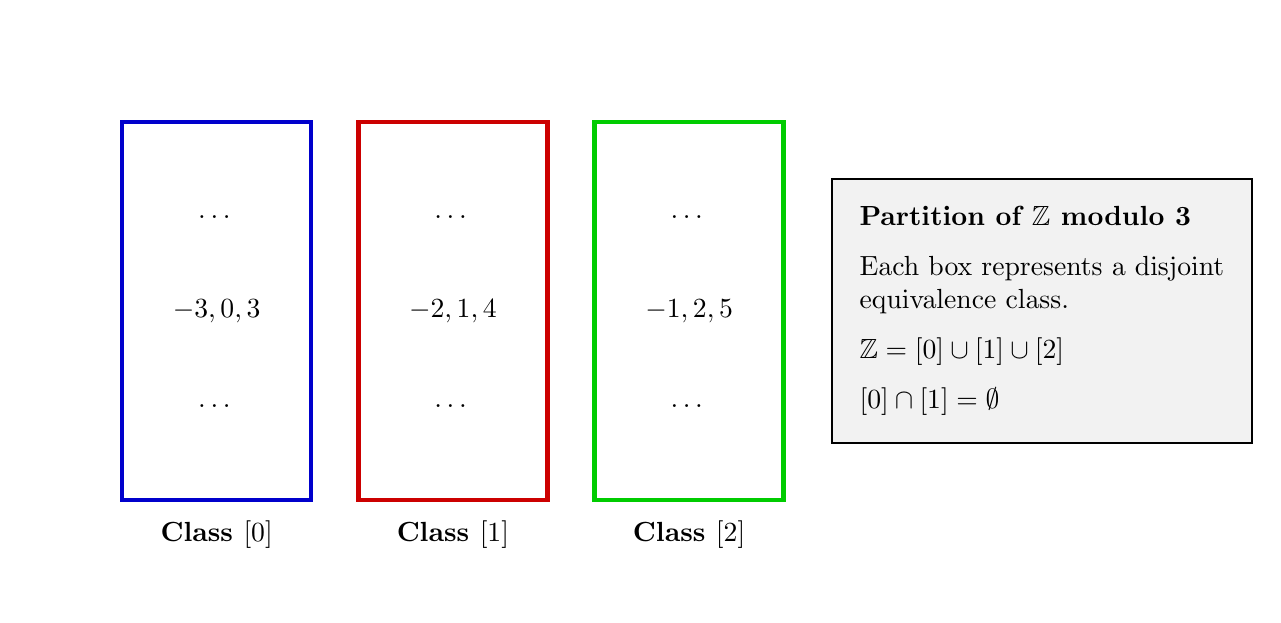
\begin{tikzpicture}[scale=1.2]
    % Background layer to ensure safe rendering
    \fill[white] (-1,-1) rectangle (9,5);
    
    % Draw the bounding boxes for the equivalence classes
    \draw[ultra thick, blue!80!black] (0,0) rectangle (2,4);
    \draw[ultra thick, red!80!black] (2.5,0) rectangle (4.5,4);
    \draw[ultra thick, green!80!black] (5,0) rectangle (7,4);
    
    % Insert the elements of the sets
    \node[black] at (1,3) {$\displaystyle \dots$};
    \node[black] at (1,2) {$\displaystyle -3, 0, 3$};
    \node[black] at (1,1) {$\displaystyle \dots$};
    
    \node[black] at (3.5,3) {$\displaystyle \dots$};
    \node[black] at (3.5,2) {$\displaystyle -2, 1, 4$};
    \node[black] at (3.5,1) {$\displaystyle \dots$};
    
    \node[black] at (6,3) {$\displaystyle \dots$};
    \node[black] at (6,2) {$\displaystyle -1, 2, 5$};
    \node[black] at (6,1) {$\displaystyle \dots$};
    
    % Labels for the classes
    \node[black, below=4pt] at (1,0) {\textbf{Class $[0]$}};
    \node[black, below=4pt] at (3.5,0) {\textbf{Class $[1]$}};
    \node[black, below=4pt] at (6,0) {\textbf{Class $[2]$}};
    
    % Single-Node Multiline Legend using Anchor Pivot
    \node[align=left, draw=black, thick, inner sep=10pt, anchor=west, fill=gray!10] at (7.5, 2) {
        \textbf{Partition of $\mathbb{Z}$ modulo 3} \\[6pt]
        Each box represents a disjoint \\
        equivalence class. \\[6pt]
        $\displaystyle \mathbb{Z} = [0] \cup [1] \cup [2]$ \\[6pt]
        $\displaystyle [0] \cap [1] = \emptyset$
    };
\end{tikzpicture}
\end{center}

\subsection{Heuristics \& Pitfalls}
\begin{itemize}
    \item \textbf{Heuristic:} When asked to find equivalence classes for a relation like $a^k \equiv b^k \pmod{n}$, do not try to solve it algebraically. Instead, compute $x^k \pmod{n}$ for $x \in \{0, 1, \dots, n-1\}$ and group the inputs that yield the same output.
    \item \textbf{Pitfall (Cancellation Fallacy):} Assuming that $ac \equiv bc \pmod{n} \implies a \equiv b \pmod{n}$ is a fatal error if $\gcd(c, n) \neq 1$. For example, $2 \cdot 3 \equiv 2 \cdot 0 \pmod{6}$, but $3 \not\equiv 0 \pmod{6}$.
\end{itemize}

\newpage
% ==========================================
% PART 5: CONCEPTUAL SYNTHESIS
% ==========================================
\section{Part 5: Conceptual Synthesis and The "Big Picture"}

\subsection{A) Thematic Connections}
The central theme of Section 9.5 is \textbf{Quotient Spaces}. By defining an equivalence relation on a large, unwieldy set (like the infinite set of integers $\mathbb{Z}$), we can "collapse" or "quotient" the set into a finite, manageable structure (like $\mathbb{Z}_n$). This process of treating "equivalent" things as "identical" is the bedrock of abstract algebra. It allows mathematicians to build new algebraic structures (groups, rings, fields) from existing ones.

\subsection{B) Forward and Backward Links}
\begin{itemize}
    \item \textbf{Backward Links:} This topic rigorously formalizes the elementary school concept of "division with remainder" (The Division Algorithm) using the language of set theory and relations.
    \item \textbf{Forward Links:} Understanding $\mathbb{Z}_n$ is the absolute prerequisite for Group Theory (studying cyclic groups), Ring Theory (ideals and quotient rings), and Topology (where equivalence relations are used to glue spaces together, e.g., creating a torus from a flat square).
\end{itemize}

% ==========================================
% PART 6: ABSTRACT REAL-WORLD MODELING
% ==========================================
\section{Part 6: Abstract Real-World Modeling (AI, ML, \& Quant Finance)}

\subsection{A) Concrete Scenarios}
\begin{enumerate}
    \item \textbf{Quantitative Finance (Monte Carlo Simulations):} Pricing complex exotic derivatives often requires simulating millions of stochastic paths. This requires massive amounts of pseudo-random numbers. Linear Congruential Generators (LCGs), which rely entirely on the properties of equivalence classes modulo a large prime $n$, are foundational algorithms for generating these uniform distributions.
    \item \textbf{Machine Learning (Hashing Algorithms):} In large-scale distributed ML (like training LLMs), data must be partitioned across thousands of GPUs. Hash functions often use modular arithmetic ($h(x) = x \pmod{n}$) to map high-dimensional data uniformly into $n$ distinct buckets (equivalence classes), ensuring balanced memory loads.
\end{enumerate}

\subsection{B) Model Problem Setup: LCG for Stochastic Path Generation}
Suppose a quantitative researcher is pricing an Asian Option and needs to simulate a Brownian Motion path $W_t$. They require a sequence of independent uniform random variables $U_i \sim \text{Uniform}(0,1)$. 

We define a state space $\mathcal{S} = \{0, 1, \dots, m-1\}$ representing the equivalence classes modulo $m$. We define a deterministic transition function $f: \mathcal{S} \to \mathcal{S}$ using an equivalence relation:
\[ \displaystyle X_{i+1} \equiv (aX_i + c) \pmod{m} \]
where $m$ is a large modulus (e.g., $2^{31}-1$), $a$ is the multiplier, and $c$ is the increment. 

The sequence of states $X_i$ maps to the continuous probability space via the transformation:
\[ \displaystyle U_i = \frac{X_i}{m} \]
For the sequence to have the maximum possible period (visiting every equivalence class exactly once before repeating), the Hull-Dobell Theorem dictates strict number-theoretic conditions based on prime factorization and divisibility—concepts directly derived from the equivalence relations studied in this chapter.

\newpage
% ==========================================
% PART 7: COMMON VARIATIONS
% ==========================================
\section{Part 7: Common Variations and Untested Concepts}

A critical concept often tested in advanced courses, but missing from this specific homework set, is proving that \textbf{arithmetic operations are well-defined on equivalence classes}. 

\textbf{Theorem:} If $a \equiv b \pmod{n}$ and $c \equiv d \pmod{n}$, then $ac \equiv bd \pmod{n}$.

\textbf{Proof:}
By definition, there exist integers $k, j$ such that:
\[ \displaystyle a = b + kn \]
\[ \displaystyle c = d + jn \]
Multiplying these equations yields:
\[ \displaystyle ac = (b + kn)(d + jn) = bd + bjn + knd + kjn^2 \]
Factoring out $n$ from the last three terms:
\[ \displaystyle ac = bd + n(bj + kd + kjn) \]
Since $(bj + kd + kjn) \in \mathbb{Z}$, it follows that $n \mid (ac - bd)$. Therefore, $ac \equiv bd \pmod{n}$. $\blacksquare$

This proof is vital because it guarantees that when we multiply two equivalence classes $[a] \cdot [c]$, the result $[ac]$ does not depend on which specific representatives $a$ and $c$ we chose from the classes.

\newpage
% ==========================================
% PART 8: ADVANCED DIAGNOSTIC TESTING
% ==========================================
\section{Part 8: Advanced Diagnostic Testing: "Find the Flaw"}

Below are five proofs related to equivalence relations and modular arithmetic. Each contains a subtle, critical flaw. Your task as the grader is to find the error.

\subsection*{Problem 1}
\textbf{Claim:} If $ac \equiv bc \pmod{n}$, then $a \equiv b \pmod{n}$. \\
\textbf{Proof:} We are given that $n \mid (ac - bc)$. Factoring out $c$, we get $n \mid c(a - b)$. Dividing both sides of the divisibility relation by $c$, we obtain $n \mid (a - b)$. Therefore, $a \equiv b \pmod{n}$. $\blacksquare$

\subsection*{Problem 2}
\textbf{Claim:} The relation $R$ on $\mathbb{Z}$ defined by $a \mathrel{R} b$ if $a + b$ is even is NOT transitive. \\
\textbf{Proof:} Assume $a \mathrel{R} b$ and $b \mathrel{R} c$. This means $a + b = 2k$ and $b + c = 2j$. Adding them gives $a + 2b + c = 2k + 2j$. Since $2b$ is even, and the right side is even, $a + c$ must be even. However, if $a=1, b=2, c=3$, then $1+2=3$ (odd), so the premise is vacuous, meaning transitivity fails in general. $\blacksquare$

\subsection*{Problem 3}
\textbf{Claim:} $a \equiv b \pmod{0}$ is a valid equivalence relation that partitions $\mathbb{Z}$ into infinite classes. \\
\textbf{Proof:} By definition, $a \equiv b \pmod{0} \iff 0 \mid (a - b)$. This means $a - b = 0 \cdot k = 0$. Thus $a = b$. This is simply the equality relation, which is reflexive, symmetric, and transitive. Therefore, it partitions $\mathbb{Z}$ into infinite classes. $\blacksquare$

\subsection*{Problem 4}
\textbf{Claim:} If $a^2 \equiv b^2 \pmod{3}$, then $a \equiv b \pmod{3}$. \\
\textbf{Proof:} We are given $3 \mid (a^2 - b^2)$. Factoring the difference of squares yields $3 \mid (a - b)(a + b)$. Since 3 is prime, Euclid's Lemma states that $3 \mid (a - b)$ or $3 \mid (a + b)$. If $3 \mid (a - b)$, then $a \equiv b \pmod{3}$. Thus the claim holds. $\blacksquare$

\subsection*{Problem 5}
\textbf{Claim:} If $a \equiv b \pmod{n}$, then $c^a \equiv c^b \pmod{n}$ for any integer $c > 0$. \\
\textbf{Proof:} Since $a \equiv b \pmod{n}$, we know $a = b + kn$. Substitute this into the exponent: $c^a = c^{b + kn} = c^b \cdot c^{kn} = c^b \cdot (c^n)^k$. By modular arithmetic properties, we can evaluate this modulo $n$. Thus, the equivalence is preserved. $\blacksquare$

\vspace{1cm}
\hrule
\vspace{0.5cm}

\subsection*{Solution Key: The Flaws Revealed}
\begin{enumerate}
    \item \textbf{Flaw in 1:} You cannot simply "divide" a divisibility relation by $c$ unless $\gcd(c, n) = 1$. If $c$ and $n$ share a factor, the modulus must also be divided by that factor. (e.g., $2 \cdot 3 \equiv 4 \cdot 3 \pmod{6}$, but $2 \not\equiv 4 \pmod{6}$).
    \item \textbf{Flaw in 2:} The counterexample provided ($a=1, b=2$) violates the initial assumption that $a \mathrel{R} b$. In logic, a conditional statement $P \implies Q$ is vacuously \textit{true} if $P$ is false, not false. The algebraic proof in the first half actually proves it \textit{is} transitive.
    \item \textbf{Flaw in 3:} While $a \equiv b \pmod{0}$ does indeed simplify to $a = b$ (the equality relation), the flaw is in the conclusion. The equality relation partitions $\mathbb{Z}$ into classes containing exactly \textit{one} element each (e.g., $[1] = \{1\}$), not infinite classes.
    \item \textbf{Flaw in 4:} The proof ignores the second outcome of Euclid's Lemma: $3 \mid (a + b)$. If $a = 1$ and $b = 2$, then $1^2 \equiv 2^2 \pmod{3}$ (since $1 \equiv 4 \pmod{3}$), but $1 \not\equiv 2 \pmod{3}$. The claim is false.
    \item \textbf{Flaw in 5:} Modular arithmetic allows substitution in the \textit{base}, not the \textit{exponent}. For example, $1 \equiv 4 \pmod{3}$, but $2^1 \not\equiv 2^4 \pmod{3}$ (since $2 \not\equiv 16 \pmod{3}$). Exponents must be evaluated modulo $\phi(n)$ (Euler's Totient Function), not modulo $n$.
\end{enumerate}

\end{document}